For our task of colorising SAR images we require an extensive dataset of paired Sentinel 1 and Sentinel 2 images. Along with the image pairs, we also require additionally metada for text conditioning during the colorisation process. This chapter delves into the extensive process of metadata choices and image acquisition.

\section{Dataset specification}

One of the most crucial information a dataset provides is the metainformation for the items in it. Therefore, we have decided on a set of information that accompanies every image provided with the dataset.

Each image in the dataset has the following common attributes:
\begin{itemize}
    \item \textbf{Coordinates:} Geo-coordinates of the top-left point of the image.
    \item \textbf{Country:} Name of the country where the image was captured.
    \item \textbf{Date-Time:} Date and time when the image was captured.
    \item \textbf{Resolution Scale:} Geospatial resolution of the image.
    \item \textbf{Temperature Region:} Temperature zone of the region in the image.
    \item \textbf{Season:} Season in the specific region at the time the image was captured.
\end{itemize}

Sentinel 1 images have two more attributes to them:
\begin{itemize}
    \item \textbf{Operational Mode:} It is the operational/acquisition mode of the satellite it used to capture the given image.
    \item \textbf{Polarisation:} It is the polarisation with which the image was captured.
\end{itemize}

Sentinel 2 images have one unique attribute:
\begin{itemize}
    \item \textbf{Bands:} Sentinel 2 images come with multiple different information channels called bands, this attribute contains a list of the bands in the image.
\end{itemize}

These were all the metadata associated with the images in the dataset. This information is later leveraged as additional information for text guidance in the colorisation process.

\section{Image acquisition}

Now, that the metadata keys have been decided, we need to select appropriate values for them. Once the values are decided, they can be used to acquire images from the ESA's Copernicus API.

\subsection{Satellite operational mode}

Sentinel‑1A and Sentinel‑1B operate using four exclusive acquisition modes: \textbf{Stripmap (SM)}, \textbf{Interferometric Wide Swath (IW)}, \textbf{Extra Wide Swath (EW)}, and \textbf{Wave (WV)}. These modes utilize the satellite’s C-SAR instrument and vary in swath width, resolution, and application.\cite{eos2024sentinel1}

\subsubsection{Stripmap (SM) Mode:}

SM mode ensures compatibility with earlier missions like ERS and Envisat. It offers high-resolution (5 x 5 m) imaging with a swath width of 80 km. The mode uses six overlapping swaths, each controlled by fixed azimuth and elevation pointing. Users can switch among beams by adjusting incidence angles and elevation beam width.


\textbf{Advantages:}
\begin{itemize}
    \item High geometric resolution suitable for detailed studies.
    \item Effective ambiguity suppression via beamforming.
\end{itemize}

\textbf{Disadvantages:}
\begin{itemize}
    \item Limited swath width.
    \item Not ideal for continuous land monitoring or large-area coverage.
\end{itemize}

\subsubsection{\textbf{Interferometric Wide Swath (IW) Mode:}}

IW mode is the primary mode for land observation. It combines a 250 km swath width with (5 x 20 m) resolution and implements the TOPS (Terrain Observation with Progressive Scans) technique, which enhances uniformity across images.

TOPSAR reduces the azimuth antenna pattern footprint by steering it opposite to the satellite’s motion. This achieves uniform Signal-to-Noise Ratio (SNR) and Distributed Target Ambiguity Ratio (DTAR), maintaining consistent image quality.

The IW mode also supports burst synchronization for interferometric applications. With Doppler and wave number spectrum overlaps, it ensures image homogeneity and phase coherence.


\textbf{Advantages:}
\begin{itemize}
    \item Balanced resolution and coverage (250 km swath).
    \item TOPSAR technique minimizes scalloping and distortion.
    \item Ideal for change detection and land deformation analysis.
\end{itemize}

\textbf{Disadvantages:}
\begin{itemize}
    \item Slightly lower resolution than SM mode.
    \item Requires high co-registration precision for interferometry.
\end{itemize}

\subsubsection{\textbf{Extra Wide Swath (EW) Mode:} }

EW mode employs the same TOPSAR principle as IW but extends the swath to 400 km using five sub-swaths. It provides a coarser resolution of 20 x 40 m and is primarily used over oceans and polar regions where spatial coverage outweighs detail.


\textbf{Advantages:}
\begin{itemize}
    \item Covers vast areas quickly.
    \item Suited for sea ice and maritime surveillance.
\end{itemize}

\textbf{Disadvantages:}
\begin{itemize}
    \item Low resolution unsuitable for terrestrial or fine-grained applications.
\end{itemize}

\subsubsection{\textbf{Wave (WV) Mode: }}

WV mode offers 20 × 20 km vignettes captured at intervals of 100 km along the satellite's path. It alternates elevation beams to provide ocean wave spectrum data using only single polarisation (HH or VV). Incidence angles range from 23° to 36.5°.


\textbf{Advantages:}
\begin{itemize}
    \item Specialized for ocean wave analysis.
    \item Provides long-duration oceanic data per orbit.
\end{itemize}

\textbf{Disadvantages:}
\begin{itemize}
    \item Inapplicable for land-based mapping.
    \item Produces small, isolated vignettes rather than continuous scenes.
\end{itemize}

\subsubsection{\textbf{Why IW Mode is Chosen: }}

The \textbf{Interferometric Wide Swath (IW) mode} stands out as the most suitable acquisition mode for land-focused applications such as SAR image colorization. Unlike the high-resolution but narrow-view SM mode, or the ultra-wide but low-resolution EW mode, IW mode achieves an optimal trade-off between spatial detail and areal coverage. Its use of the TOPSAR scanning technique results in uniform signal and image quality across the entire swath, crucial for generating high-fidelity datasets needed in downstream image translation or enhancement tasks.

Additionally, IW mode is tailored to support coherent radar change detection and interferometry by ensuring spectral overlap and burst synchronization. These capabilities are vital when aligning SAR images with optical references like Sentinel‑2, as they maintain geometric consistency and temporal coherence. Therefore, considering both technical robustness and operational balance, IW mode is best suited for acquiring Sentinel-1 data for land monitoring and image enhancement tasks.



\subsection{Polarization}

Synthetic Aperture Radar (SAR) imaging onboard Sentinel-1 supports multiple polarisation modes, allowing the radar to transmit and receive signals in both vertical and horizontal orientations. These configurations include \textbf{VV}, \textbf{VH}, \textbf{HH}, and \textbf{HV}. In the Interferometric Wide (IW) swath mode, Sentinel-1 satellites primarily offer the \textbf{VV} and \textbf{VH} dual-polarisation configuration. Each polarisation setup exhibits unique imaging behaviors depending on the physical properties of the Earth's surface.

\subsubsection{\textbf{VV Polarisation (Vertical transmit – Vertical receive):}}

In this configuration, the radar pulses are emitted with a vertical orientation and the sensor records vertically polarised echoes. This mode is particularly effective at capturing reflections from flat surfaces or structures with strong angular edges, such as urban environments. The double-bounce effect between ground and building walls often enhances the backscattering response in VV mode. Additionally, open terrain and bare soil produce strong surface scattering under this setup.


\textit{Advantages:}
\begin{itemize}
    \item Produces strong backscatter in man-made environments and smooth terrains.
    \item Excellent for distinguishing water bodies due to their specular reflection producing low return (dark pixels).
    \item Relatively noise-resilient and more consistent across different land surfaces.
\end{itemize}

\textit{Disadvantages:}
\begin{itemize}
    \item Struggles to capture volume scattering features such as dense vegetation.
    \item Less sensitive to canopy and biomass density compared to cross-pol modes.
\end{itemize}

\subsubsection{\textbf{VH Polarisation (Vertical transmit – Horizontal receive):}}

This configuration involves the transmission of vertically polarised waves and reception of horizontally polarised ones. VH is a cross-polarisation mode that captures volume scattering effectively. It is more responsive to randomly oriented scatterers, such as leaves, branches, or forest canopies, making it useful for distinguishing vegetated regions.


\textit{Advantages:}
\begin{itemize}
    \item Highly sensitive to vegetation structure and density.
    \item Improves discrimination between built-up areas and natural surfaces when used alongside VV in dual-pol mode.
\end{itemize}

\textit{Disadvantages:}
\begin{itemize}
    \item Yields weaker returns from surfaces with minimal volumetric complexity (e.g., bare soil, urban surfaces).
    \item Lower signal-to-noise ratio in comparison to co-polarisation.
\end{itemize}

\subsubsection{\textbf{HH Polarisation (Horizontal transmit – Horizontal receive):}}

In this co-polarisation mode, the system transmits and receives radar signals in the horizontal direction. Though not supported in IW mode of Sentinel-1, this mode has demonstrated utility in sea-ice monitoring and agricultural applications in other SAR missions.


\textit{Advantages:}
\begin{itemize}
    \item Effective for ocean surface observations under specific environmental conditions.
    \item Can highlight rougher surface scattering on water or snow.
\end{itemize}

\textit{Disadvantages:}
\begin{itemize}
    \item Not supported in IW mode of Sentinel-1.
    \item Offers limited benefit for land use classification compared to VV/VH.
\end{itemize}

\subsubsection{\textbf{HV Polarisation (Horizontal transmit – Vertical receive):}}

Similar to VH, this cross-polarised mode is not enabled in IW acquisitions for Sentinel-1. However, in missions that do offer it, HV behaves similarly to VH, revealing internal vegetation structures and terrain volume complexity.


\textit{Advantages:}
\begin{itemize}
    \item Useful in forestry studies for identifying canopy features and forest degradation.
\end{itemize}

\textit{Disadvantages:}
\begin{itemize}
    \item Not available in Sentinel-1 IW mode.
    \item Lower signal strength compared to co-polar modes.
\end{itemize}

\subsubsection{\textbf{Why VV + VH polarization mode ?}}

Given the operational limitations and application scope, the dual-polarisation configuration of \textbf{VV + VH} stands out as the most balanced and informative mode for Sentinel-1 IW data. VV enables clear imaging of built-up surfaces, bare land, and water bodies, while VH supplements this by providing crucial information on vegetative structures. Together, they offer complementary insights across a range of land cover types, making this dual-pol setup optimal for most earth observation and land use applications where SAR imaging is applied.



\subsection{Resolution Scale}

10m

\subsection{Season Classification}

Now, it is needed to classify the season for an image depending on its country and the timestamp from when the image was captured. To do so, we will need seasonal duration data for all countries. This information is not always available for all countries. Also, the seasons are not always the same 4 seasons for all countries, especially given current circumstances with global climate. Hence we need to devise a standardised method to classify seasons for various countries into the four major seasons: \textbf{Winter}, \textbf{Spring}, \textbf{Summer}, and \textbf{Fall}.

To perform this task, we devised an algorithm. It goes as follows:
\begin{enumerate}
    \item Acquire a list of all countries along with a few cities from each country. This is done by using the Simple Maps World Cities dataset\cite{world_cities}. This dataset contains a list of 248 countries along with a few cities from each country and their coordinates.
    \item Retrieve historical weather data (daily average temperature) for a span of a year for every city under each country. This data is retrieved from Open-Meteo\cite{Zippenfenig_Open-Meteo} which provides free API access for various categories of weather data.

    Relevant code snippet can be found in Appendix A. Listing \ref{code:season}.
    \item Average the temperature across all cities for a country to find the daily average temperature of the country over a year.
    \item Find maximum temperature and minimum temperature for each country. This information will be used to calculate time periods for the seasons. It is done in the following way:
    \begin{itemize}
        \item The maximum temperature is considered the peak of summer and the minimum temperature is considered the trough of winter.
        \item The temperatures have an accuracy of 9 significant figures after decimal, so chances of collision (ie., two or more peaks or trough) is almost negligible. Yet, to account for collision, we need to check the hemisphere information.

        If the country is in northern hemisphere, Choose the first peak and trough and vice-versa for southern hemisphere. The reasoning behind this is the general opposite climate in both the hemispheres.
        \item We find the difference between the temperatures, consider it \textit{D}.
        \item Consider \textit{D/4} temperature difference from maximum temperature the onset and end of summer, the same goes for the \textit{D/4} temperature difference from winter. This temperature is called the \textit{transition point}.
        \item Traverse through days towards the past from peak temperature to find a day that has the \textit{transition point} temperature. This is end of spring. Traversing towards future from trough will give us the onset of spring. Similarly in the opposite manner we can fine onset and end of fall.
        \item To find this day, we include a buffer period of 7 days before matching temperature. This is to ensure that a season lasts at least for the duration of a week.
    \end{itemize}
    \item Thus we now have seasonal data for every country.
    \item For contingency, for any country whose data could not be calculated will rely on the classical meteorological season segragation.
\end{enumerate}

This seasonal classification data is later used to map the season metadata value for images.

\subsection{Temperature Region Classification}

Temperature regions are also known as heat zones of the Earth. There are three heat zones, Arctic or Frigid zone, Temperate zone, and Tropical or Torrid Zone. These zones are classified according to latitude.

\begin{itemize}
    \item Tropical Zone: It lies between the Tropic of Cancer ($23.5^\circ$ North) and Tropic of Capricorn ($23.5^\circ$ South). This zone receives the most heat from the sun.
    \item Temperate Zone: In the northern hemisphere, this zone lies between Tropic of Cancer and the Arctic circle ($66.5^\circ$ North). In the southern hemisphere, it lies between Tropic of Capricorn and Antarctic circle ($66.5^\circ$ South).This region is moderately cooler compared to the tropical region.
    \item Arctic Zone: In the northern hemisphere, it is located between the North Pole ($90^\circ$ North) and Arctic circle. In the southern hemisphere, it lies between the South Pole ($90^\circ$ South) and the Antarctic circle. This region is the coldest region of them all.
\end{itemize}

Temperature region data is included in the metadata with the images.

\subsection{Copernicus API}

Copernicus Data Space Ecosystem with a tagline of Europe's eyes on Earth is an open ecosystem that provides free instant access to a wide range of data and services from the Copernicus Sentinel missions\cite{copernicusHome}. It provides data from all Sentinel satellites in various forms.

For Sentinel 1 images we used the "Level 1 Ground Range Detected (GRD)" collection and for Sentinel 2 images we used "Level 3 Monthly Mosaics" collection. The following sections contain an overview of how the copernicus API was used to obtain the images for the dataset.

\subsubsection{Generating coordinates}

Coordinates are generated randomly over the world but are majorly limited to landmass only with a few coastline data. The reason for being majorly landmass is that, the major SAR usefulness comes from it imaging landmass data through clouds. For ocean or water body data, SAR imaging is not used, rather high resolution optical images are used.

The random landmass coordinates are generated from Natural Earth Land Data\cite{naturalearthland}. And the coastline data are generated from Natural Earth Coastline Data\cite{naturalearthcoast}.

The Copernicus service provides a limited number of API calls per month for free users (30,000 calls). To maximize efficiency of API call usage, we decided to obtain images of the maximum size limit offered by Copernicus. The maximum limit is $2500\times2500$ pixels per image. But we cannot evenly divide this image into $256\times$ subsections. Thus the maximum resolution we can have is $2304\times2304$. Now, the scale of images need to be 10m.

\begin{align*}
    \text{Hence, ground distance per pixels} &= 10m \\
    \text{Total distance for 2500x image is} &= 10\times2304 \\
    &= 23,040m
\end{align*}

Thus, we need to create square patches with 23.04 KM distances as the side of the said patch. For this task, we take the randomly generated coordinates and calculate the subsequent latitude and longitude coordinates beginning from that for a consecutive 3 patches. The formulas for approximately converting longitude and latitude into kilometers are as follows:

\begin{itemize}
    \item \textbf{Latitude: } $1^\circ = 110.574$KM
    \item \textbf{Longitude:} $1^\circ = 111.320\times cos(latitude)$ KM
\end{itemize}

Thus, we end up with a list of coordinates for all regions.

\subsubsection{Defining Image Properties}

First we need to do authentication and then, the image properties are set in preparation of the image download. This is where the difference in obtaining Sentinel-1 and Sentinel-2 images appear due to differences in image formats.

We set the image height and width to 2500 pixels each. Following that, the eval script is set. An eval script is a piece of Javascript code which defines how the satellite data shall be processed by Sentinel Hub\cite{evalDoc}. Two different eval scripts are used for Sentinel-1 and Sentinel-2 images due to the different number of bands being used in the images.

The Sentinel-1 eval script is as follows:

\begin{lstlisting}[language=Java]
    //VERSION=3
    function setup() {
        return {
            input: ["VV"],
            output: { id: "default", bands: 1 }
        };
    }

    function evaluatePixel(sample) {
        return [2 * sample.VV];
    }
\end{lstlisting}

The Sentinel-2 eval script is as follows:

\begin{lstlisting}[language=Java]
    //VERSION=3
    function setup() {
        return {
            input: ["B02", "B03", "B04"],
            output: { bands: 3 }
        };
    }

    function evaluatePixel(sample) {
        return [2.5 * sample.B04/10000, 2.5 * sample.B03/10000, 2.5 * sample.B02/10000];
    }
\end{lstlisting}

From the eval scripts we can infer that Sentinel-1 images have one band, called "VV". It is the polarization of the captured image. "VV" is vertical polarization, i.e.,  vertically transmit and vertically receive. And Sentinel-2 images have 3 bands, namely, B02, B03, B04. The bands are for Blue, Green, and Red channel respectively. The Sentinel-2 images are also preprocessed before download by scaling and normalizing the pixel values. 

Then, bounding box coordinates and time frame for images are sent with the request along with the previously mentioned data.

\subsection{First Manual Inspection}

Once the images are downloaded, the first manual inspection is performed. We check the pair of images to verify that the images contain visible patterns and variations throughout its entirety. Images which had regions of no variation were discarded.

\subsection{Cropping Images}

After the first manual inspection, the images were cropped and divided into multiple smaller images to the decided resolution. The downloaded images have a dimension of $2304\times2304$ pixels. They are divided into 81 $256\times256$ sized images each.

\subsection{Second Manual Inspection}

Once the images are cropped and divided into smaller images, one last manual inspection is performed. The purpose of this inspection is the same as the first manual inspection, to verify variations in images. This check is performed to ensure no plain images exist in the dataset.

\subsection{Pre-Processing}

Now, we have arrived at one of the most important steps in dataset preparation. Pre-processing of the images in the dataset. Right from the beginning, there are two issues that remote sensing images face, namely, \textbf{Geometric Distortions due to tilt} and \textbf{Speckle noise}. The fixes for this are applied ath the sentinel hub by mentioning these fixes in the request body (See appendix \ref{code:sen1req}). To fix these issues we tackle them in the following ways:

\subsubsection{Orthorectification}

The topographical variations in the surface of the earth and the tilt of the satellite or aerial sensor can affect the distance with which features on the satellite or aerial image are displayed. The more topographically diverse the landscape, the more distortion inherent in the image.

Image data acquired by satellite or aircraft are affected by a systematic sensor and platform-induced geometry errors, which introduce terrain distortions when the sensor is not pointing directly at the Nadir location of the sensor (As is the case with sentinel satellites).

To accurately remove the image distortions, a digital elevation model (DEM) is used to perform image orthorectification. The required DEM is generated by feature extraction from high-resolution stereo satellite imagery. We use the copernicus DEM 30m datafor the purpose of orthorectification.

\subsubsection{Speckle filtering}

When a radar illuminates a surface that is rough on the scale of radar wavelength, the return signal consists of waves reflected from many elementary scatterers within a resolution cell. The distances between the elementary scatterers and the receiver vary due to the surface roughness, and, therefore, the receieved waves, although coherent in frequency, are no longer coherent in phase. A strong signal is received, if the waves add relatively constructively; a weak signal, ifthe waves are out of phase. A SAR image is formed by coherently processing the returns from successive radar pulses. This eddect causes a pixel to pixel variation in intensity, and this variation manifests itself as a granular pattern, called speckle\cite{SpeckleLee}.

To filter out speckles, we use Lee method of speckle filtering. It employs a sample mean and variance of pixels in scanning window going over the image.

\subsection{Organizing and Dataset Structure}

After acquiring all the images and processing them, they are segregated into folders based on their initial location or region. Each region folder has two subfolders that store the Sentinel 1 images and Sentinel 2 images. The root of the dataset folder also has CSV files corresponding to each region which holds the metadata for all image pairs within a given region.

Our dataset has images spread uniformly across all over the world with 165 regions and 129,438 pairs of images. Thus the total number of image files in the dataset amounts to 258,876 images. An overview of the selected regions given on the worldmap is given in Fig \ref{fig:map}

\begin{figure*}
    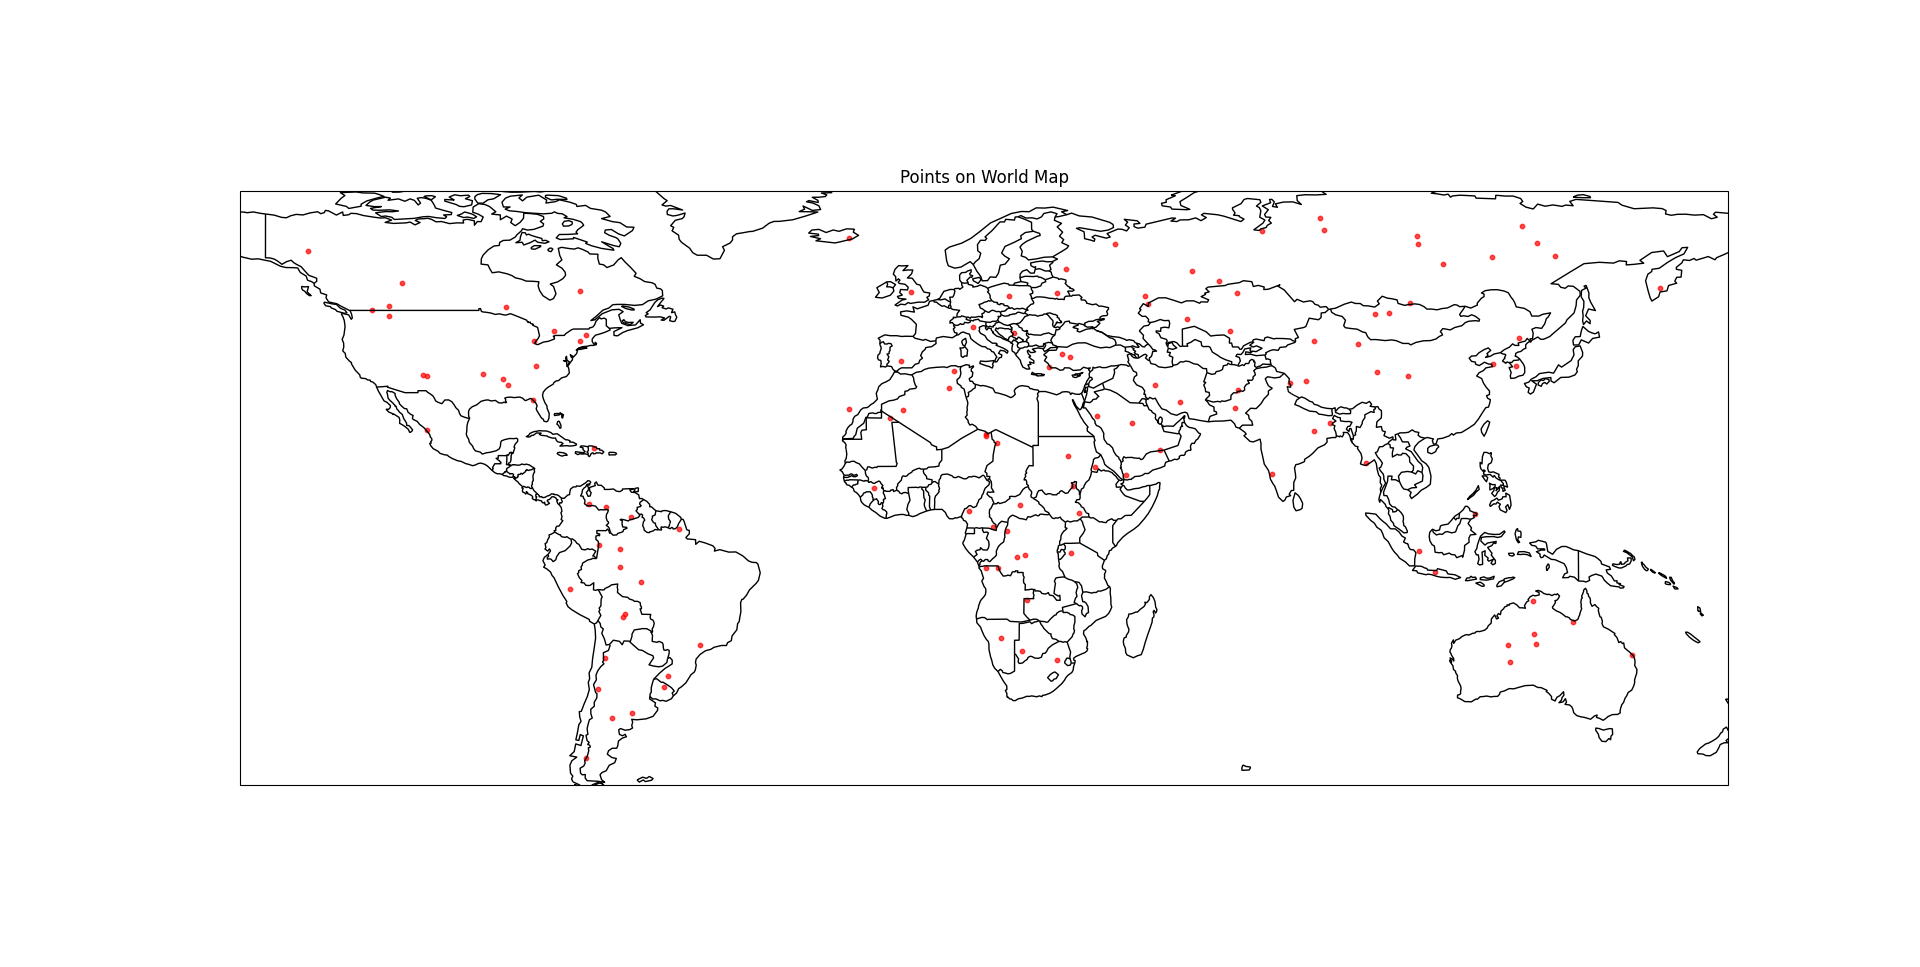
\includegraphics[width=\textwidth]{region_plot.png}
    \caption{All regions from where data has been included in the dataset}
    \label{fig:map}
\end{figure*}

A sample showcase of images from the dataset can also be seen in Fig \ref{fig:showcase}

\begin{figure*}
    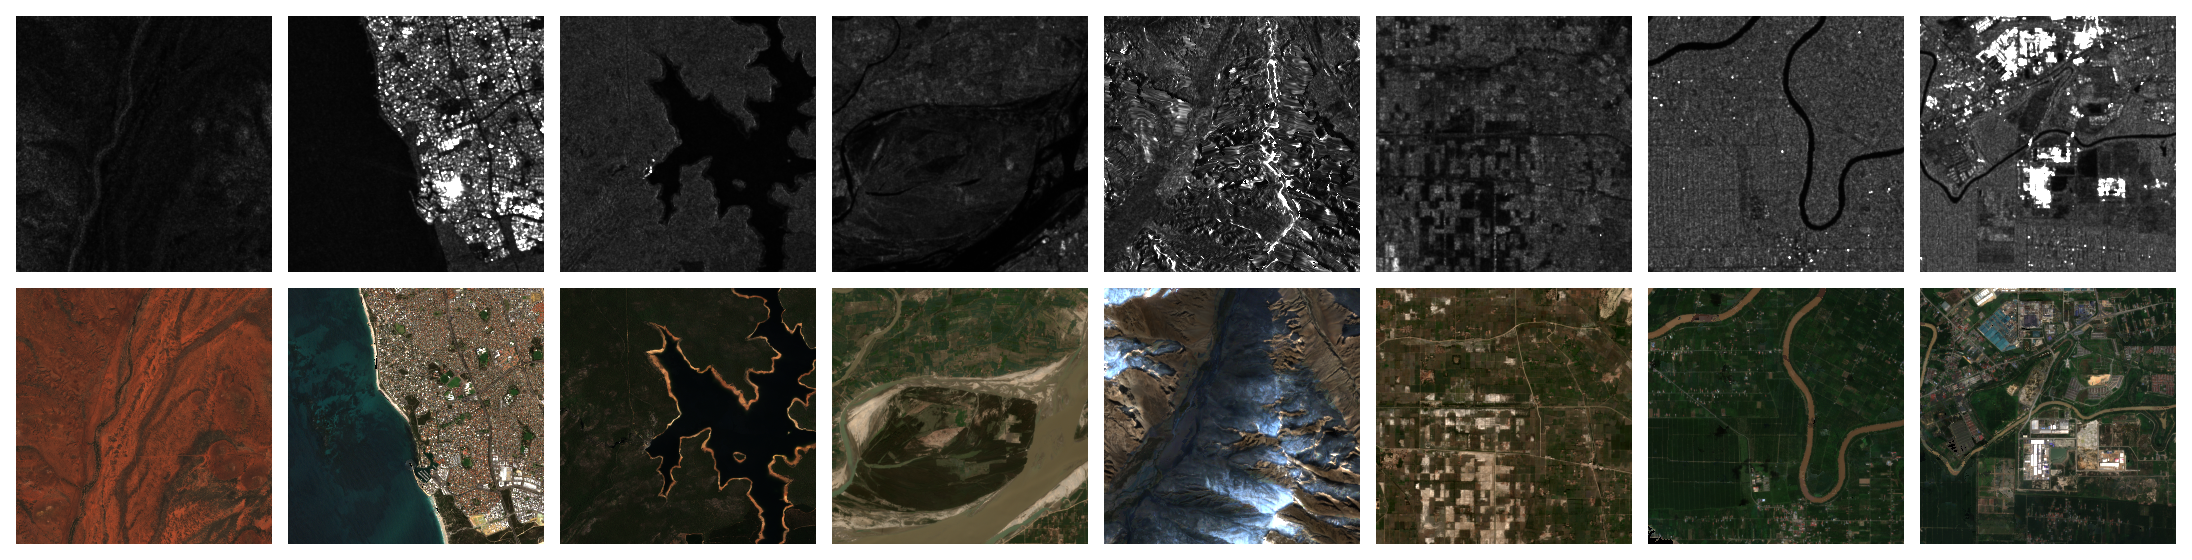
\includegraphics[width=\textwidth]{showCase.png}
    \caption{Sample images from the dataset. Top row: Sentinel-1 images, bottom row: corresponding Sentinel-2 images}
    \label{fig:showcase}
\end{figure*}

\subsection{Dataset availability}
The \textit{Uniform Sen 1-2} dataset is shared under the open access license CC-BY-SA 4.0 and is available to download at kaggle. The dataset can be accessed at \url{https://www.kaggle.com/datasets/shambac/uniform-sen-1-2-dataset}. As an when a DOI is generated for the dataset, the paper will be updated to reflect the same.